%
% fig-hankelkontur.tex
%
% (c) 2026 Prof Dr Andreas Müller
%
\begin{figure}
\centering
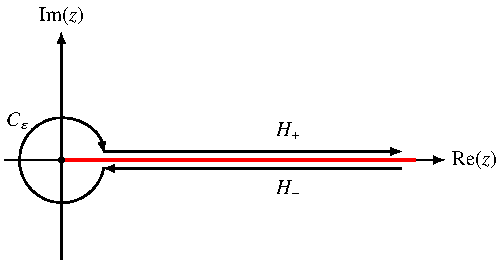
\includegraphics{papers/hankel/images/hankelkontur.pdf}
%\begin{tikzpicture}[scale=1.2,>=latex]
%	% Achsen
%	\draw[->] (-0.8,0) -- (5.4,0) node[right] {$\Re(z)$};
%	\draw[->] (0,-1.4) -- (0,1.8) node[above] {$\Im(z)$};
%	\draw[very thick,red] (0,0) -- (5.0,0);
%	% Parameter
%	\def\eps{0.6}
%	
%	% oberer und unterer Teil der Hankel-Kontur
%	\draw[->,thick] (\eps,0.12) -- (4.8,0.12);
%	\draw[->,thick] (4.8,-0.12) -- (\eps,-0.12);
%	
%	% kleiner Kreis um 0
%	\draw[<-,thick] (\eps,0.1) arc[start angle=10,end angle=350,radius=\eps];
%	
%	% Ursprung
%	\fill (0,0) circle[radius=1.2pt];
%	
%	\node[above] at (3.2,0.18) {$H_+$};
%	\node[below] at (3.2,-0.18) {$H_-$};
%	\node[left] at (-0.35,0.55) {$C_\varepsilon$};
%\end{tikzpicture}
\caption{Die Hankel-Kontur um den positiven Verzweigungsschnitt.}
\label{hankel:fig:hankelkontur}
\end{figure}
